% Copyright 2013 Nicolai Hähnle <nhaehnle@gmail.com>
%
% This work is licensed under the Creative Commons Attribution-ShareAlike 3.0
% Unported License, see http://creativecommons.org/licenses/by-sa/3.0/
%
% Among other things, this means that yes, you may take e.g. illustrations from
% the book and use them in your own work. However, (a) you must give proper
% attribution by naming me as its original author and (b) you must make your
% derivative work available under the same or similar license terms.
%
% See the Creative Commons website for the exact licensing terms.

\chapter{Generating Functions and the Algebra of Polyhedra}

We have seen how to enumerate the lattice points in a convex body $K$
in time that is essentially proportional to the maximum number of lattice points
in a translate of $K$.
What if we are only interested in the \emph{number} $|K \cap \Lambda|$ of such points?

Throughout this chapter, we will work with $\Lambda = \Z^d$ -- using a linear transformation,
this is without loss of generality.
Consider the box $K = [0,M]^d$.
It contains roughly $M^d$ integer points, which is exponential in the number of bits
required to encode a description of $K$.
On the other hand, computing this number is a trivial task that can be performed in
polynomial time in the encoding length of $K$.
This leads us to suspect that \emph{computing the number} of integer points could be
exponentially faster than \emph{enumerating} all those points.

In the case of a box,
computing the number of points is a polynomial problem even when the dimension $d$ is allowed to vary.
We do not expect this to be true in general
because the problem of deciding whether $|P \cap \Z^d|$ is $0$ for an arbitrary polytope $P$ is the integer programming problem,
which is $NP$-hard.
In fact, computing $|P \cap \Z^d|$ is easily seen to be a $\# P$-hard problem.
So we should contend ourselves with looking for an algorithm that is polynomial so long as $d$ is fixed,
and with trying to reduce the dependence on $d$ of the degree of this polynomial.

The enumeration algorithms of the last chapter could be formulated with representations of convex bodies via oracles.
This is no longer the case for computing the number of integer points.
Let $N \in \N$ and consider the convex body
\[
  K_\varepsilon(a,b) := \{ (x,y) \in \R^2 ~:~ a \leq x \leq b, xy \geq N + \varepsilon, y \leq N \}
\]
The lower envelope of $K_0(a, b)$ contains an integer point if and only if $N$ has a factor between $a$ and $b$,
see Figure~\ref{fig:factoring-body}.
Consequently, for $\varepsilon \in (0,1)$ one has $|K_0 \cap \Z^2| - |K_\varepsilon \cap \Z^2| > 0$ if and only if $N$ has a factor between $a$ and $b$.
\begin{fact}
  If there were a polynomial-time algorithm for computing the number of integer points in (somewhat general) convex bodies in $\R^2$,
  then one could factor integers in polynomial time.
\end{fact}
We don't expect factoring to be a polynomial time problem,
so we cannot hope to count integer points in arbitrary convex bodies.
Instead, our goal will be a polynomial time algorithm that counts the number of integer points in \emph{polytopes}
in fixed dimension.

\begin{figure}
  \begin{center}
    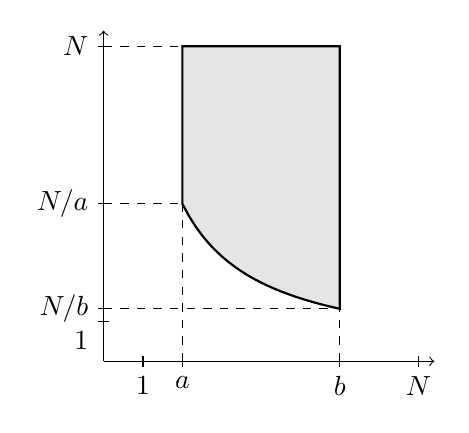
\begin{tikzpicture}
      \draw[->] (0,0) -- (4.2,0);
      \draw[->] (0,0) -- (0,4.2);
      
      \draw[dashed] (0,0.666) -- (3,0.666);
      \draw[dashed] (0,2) -- (1,2);
      \draw[dashed] (0,4) -- (1,4);
      
      \draw[dashed] (1,0) -- (1,2);
      \draw[dashed] (3,0) -- (3,0.666);

      \draw (0.5,0) +(0,2pt) -- +(0,-2pt) node[below] {$1$};
      \draw (1,0) +(0,2pt) -- +(0,-2pt) node[below] {$a$};
      \draw (3,0) +(0,2pt) -- +(0,-2pt) node[below] {$b$};
      \draw (4,0) +(0,2pt) -- +(0,-2pt) node[below] {$N$};
      \draw (0,0.5) +(2pt,0) -- +(-2pt,0) node[below left] {$1$};
      \draw (0,2) +(2pt,0) -- +(-2pt,0) node[left] {$N/a$};
      \draw (0,0.666) +(2pt,0) -- +(-2pt,0) node[left] {$N/b$};
      \draw (0,4) +(2pt,0) -- +(-2pt,0) node[left] {$N$};
      
      \draw[thick,fill=black!10] plot[domain=1:3] (\x, {2 / \x}) -- (3,4) -- (1,4) -- cycle;
    \end{tikzpicture}
  \end{center}
  \caption{The body $K_0(a,b)$ encodes information about the factors of $N$.}
  \label{fig:factoring-body}
\end{figure}



\section{A simple example of generating functions}

Suppose we want to count the number of integer points in an interval $I := [a,b] \subset \R$
in a way that might be extendable to higher dimension.
One way of doing this is to symbolically determine the \emph{generating function}
\[
  f(I;x) = \sum_{p \in I \cap \Z} x^p
\]
and evaluate it at the point $f(I;1) = |I \cap \Z|$.
Unfortunately, $f(I;x)$ is the sum of $|I \cap \Z|$ monomials.
The memory space required for writing this sum down is therefore exponential in the encoding length of $I$.
A better approach is needed. The geometric series
\[
  \sum_{p = 0}^\infty x^p
\]
is at the same time the generating function for the unbounded interval $[0,\infty)$
and satisfies
\[
  \sum_{p = 0}^\infty x^p = \frac{1}{1 - x}
\]
where the series converges absolutely.
The following picture suggest a way to leverage the geometric series for our problem:
\begin{center}
  \begin{tikzpicture}
    \draw (-0.2,0) -- (8.2,0);
    \foreach \x in {0,0.5,...,8.01}
      \draw (\x,0) +(0,2pt) -- +(0,-2pt);
    
    \draw[very thick] (2,0) node[below] {$a$} -- node[above] {$I$} (5,0) node[below] {$b$};
    
    \draw (2,-1) +(0,2pt) -- +(0,-2pt) +(0,0) -- (8.2,-1);
    \draw (5.5,-1.5) +(0,2pt) -- +(0,-2pt) +(0,0) -- (8.2,-1.5);
    
    \draw (1,-1) node {$=$};
    \draw (1,-1.5) node {$-$};
  \end{tikzpicture}
\end{center}
The graphical ``formula'' carries over to formal Laurent series (assuming $a, b \in \Z$ for simplicity):
\[
  \sum_{p = a}^b x^p = \sum_{p = a}^\infty x^p - \sum_{p = b+1}^\infty x^p
\]
There is an open set $U \subset \C$ on which all series converge absolutely,
and so
\[
  \sum_{p = a}^b x^p = \frac{x^a}{1 - x} - \frac{x^{b + 1}}{1 - x}
\]
holds on $U$.
Since the functions involved in this equation are rational and therefore complex differentiable,
it follows that the equality must hold on all of $\C$ (except for $x = 1$, where the functions are not defined).
That is, we can write
\[
  f(I;x) = \frac{x^a}{1 - x} - \frac{x^{b + 1}}{1 - x}
\]
if we understand the equality to be up to negligible differences in the domains of the two sides of the equation.
Observe that the encoding length of the right hand side is dominated by the encodings of $a$ and $b$,
and is therefore linear in the encoding length of $I$.

The downside of this representation of $f(I;x)$ is that it is undefined at $x = 1$,
which is exactly the point where we would like to evaluate it.
However, $x = 1$ is a removable singularity.
Using the rule of de~l'Hôpital, we can compute
\[
  \lim_{x \to 1} \frac{x^a}{1 - x} - \frac{x^{b + 1}}{1 - x} = \lim_{x \to 1} \frac{x^a - x^{b+1}}{1 - x} = \lim_{x \to 1} \frac{a x^{a-1} - (b+1) x^b}{-1} = b - a + 1,
\]
which is the correct answer, as the derivation above has already shown.

Note that the graphical formula we used to derive the rational generating function for $I$ is by no means unique.
The following picture shows an alternative formula:
\begin{center}
  \begin{tikzpicture}
    \draw (-0.2,0) -- (8.2,0);
    \foreach \x in {0,0.5,...,8.01}
      \draw (\x,0) +(0,2pt) -- +(0,-2pt);
    
    \draw[very thick] (2,0) node[below] {$a$} -- node[above] {$I$} (5,0) node[below] {$b$};
    
    \draw (2,-1) +(0,2pt) -- +(0,-2pt) +(0,0) -- (8.2,-1);
    \draw (-0.2,-1.5) -- (5,-1.5)  +(0,2pt) -- +(0,-2pt);
    \draw (-0.2,-2) -- (8.2,-2);
    
    \draw (-1,-1) node {$=$};
    \draw (-1,-1.5) node {$+$};
    \draw (-1,-2) node {$-$};
  \end{tikzpicture}
\end{center}
Again, this carries over to formal Laurent series:
\[
  \sum_{p = a}^b x^p = \sum_{p = a}^\infty x^p + \sum_{p = -\infty}^b x^p - \sum_{p = -\infty}^\infty x^p
\]
There are two problems:
\begin{itemize}
  \item The first two series on the right hand side are geometric series for which a rational function expression is known.
    However, their regions of absolute convergence are disjoint.
  
  \item The last series does not converge anywhere, and it is unclear what rational function expression could be used in its place.
\end{itemize}
Over the course of this chapter,
we will see that the first problem turns out not to be a problem after all,
and that the last, non-converging series, magically disappears.
One finds that
\[
  f(I;x) = \frac{x^a}{1-x} + \frac{x^b}{1-x^{-1}}
\]
where, again, the equality should be understood modulo negligible differences in the functions' domains.
For now, the reader may want to convince themselves that the equation holds in this particular example,
for example by manual comparison to the rational function obtained previously.

The remainder of this chapter generalizes the approach we have just laid out to higher dimension,
exploring some rather fascinating algebraic structures on the way.



\section{Cones and triangulations}

\begin{definition}
  \begin{enumerate}[(a)]
    \item A non-empty convex set $K \subseteq \R^d$ is a \emph{cone}
      if $p \in K$ and $\lambda \geq 0$ imply $\lambda p \in K$.
  
    \item A \emph{conic combination} of vectors $u_1, \ldots, u_n \in \R^d$ is
      a linear combination with non-negative coefficients.
  
    \item Given $U \subset \R^d$, the set $\cone(U)$ is the set of conic combinations of vectors in $U$.
  
    \item A cone $K$ is \emph{polyhedral} if $K$ is a polyhedron.
  \end{enumerate}
\end{definition}

Note that cones are closed under taking conic combinations,
and $\cone{U}$ is the smallest cone containing $U$.

\begin{definition}
  Let $P$ be a non-empty polyhedron.
  The \emph{lineality space} of $P$ is
  \[
    L(P) := \{ v \in \R^d ~:~ \forall x\in P \,\forall \lambda \in \R:~ x + \lambda v \in P  \}
  \]
\end{definition}

It is not difficult to check that $L(P)$ is a linear subspace of $\R^d$.
Intuitively, $L(P)$ contains the directions of lines contained in $P$.
Polyhedra containing lines are somewhat unusual in the sense
that if one thinks of polyhedra, one usually thinks of polyhedra that have vertices,
and such polyhedra \emph{do not} contain lines.
That is, their lineality space is $0$.
However, their properties are crucial for the development of compact rational generating functions.

The following facts tie cones, polarity, and lineality spaces together.
Their proofs are left as an exercise.

\begin{lemma}
  Let $K \subseteq \R^d$ be a closed cone.
  \begin{enumerate}[(a)]
    \item $K^\star = \{ y \in \R^d ~:~ y^Tx \leq 0 \,\forall\, x\in K \}$.
    \item $K^\star$ is a cone and $(K^\star)^\star = K$.
    \item $d = \dim L(K) + \dim K^\star$.
  \end{enumerate}
\end{lemma}

\begin{definition}
  A cone $K$ is \emph{simplicial} if $K = \cone\{ u_1, \ldots, u_k \}$ for linearly independent vectors $u_j \in \R^d$.
\end{definition}

\begin{definition}
  Let $K \subset \R^d$ be a full-dimensional simplicial cone,
  $K = \cone\{ u_1, \ldots, u_d \}$
  with $u_j \in \Z^d$ primitive integer vectors.
  Then the \emph{determinant} of $K$ is
  \[
    \det(K) := |\det(u_1,\ldots,u_d)|
  \]
  A \emph{unimodular} cone is a full-dimensional simplicial cone with determinant $1$.
\end{definition}

Again, the proofs of the following facts about simplicial and unimodular cones are left as an exercise.

\begin{lemma}
  Let $K = \cone\{u_1,\ldots,u_d\} \subset \R^d$ be a full-dimensional simplicial cone.
  \begin{enumerate}[(a)]
    \item Let $A = (u_1, \ldots, u_d)$. Then $K = \{ p \in \R^d ~:~ -A^{-1} p \leq 0 \}$.
    \item $K^\star$ is simplicial.
    \item $K$ is unimodular if and only if $K^\star$ is unimodular.
  \end{enumerate}
\end{lemma}

\begin{figure}
  \begin{center}
    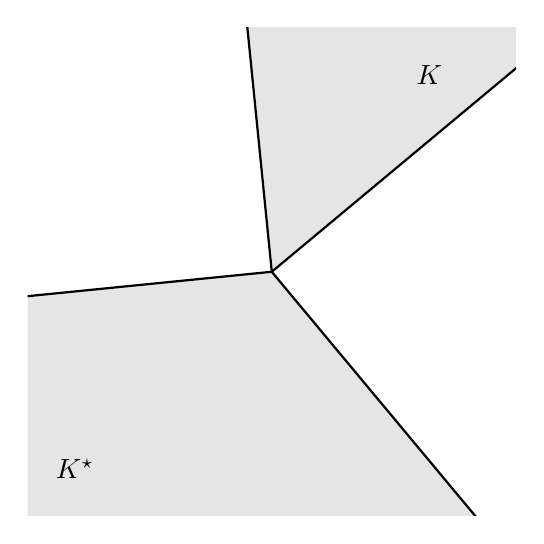
\begin{tikzpicture}
      \clip (-3.1,-3.1) rectangle (3.1,3.1);
      
      \draw[thick,fill=black!10] (-0.5,5) -- (0,0) -- (6,5);
      \draw[thick,fill=black!10] (-10,-1) -- (0,0) -- (10,-12);
      \draw (2,2.5) node {$K$};
      \draw (-2.5,-2.5) node {$K^\star$};
    \end{tikzpicture}
  \end{center}
  \caption{A simplicial cone and its polar.}
\end{figure}


Working with simplicial cones is desirable due to their simple combinatorial structure.
For this reason, we want to \emph{triangulate} more complicated polyhedral cones into simplicial cones.
We start by defining the notion of triangulation for polytopes,
see Figure~\ref{fig:triangulation-example}.

\begin{definition}
  Let $P \subset \R^d$ be a polytope.
  A set of simplices $\Delta_1, \ldots, \Delta_n$ is a \emph{triangulation} of $P$ if
  \begin{enumerate}
    \item $P = \bigcup_j \Delta_j$ and
    \item for every $i \neq j$, $\Delta_i \cap \Delta_j$ is a face of both $\Delta_i$ and $\Delta_j$ (possibly the empty face).
  \end{enumerate}
\end{definition}

\begin{figure}
  \begin{center}
    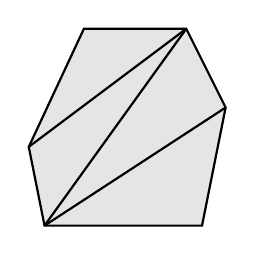
\begin{tikzpicture}
      \coordinate (n1) at (0,0);
      \coordinate (n2) at (2,0);
      \coordinate (n3) at (2.3,1.5);
      \coordinate (n4) at (1.8,2.5);
      \coordinate (n5) at (0.5,2.5);
      \coordinate (n6) at (-0.2,1);
      
      \draw[thick,fill=black!10] (n1) -- (n2) -- (n3) -- (n4) -- (n5) -- (n6) -- cycle;
      \draw[thick] (n1) -- (n3);
      \draw[thick] (n1) -- (n4);
      \draw[thick] (n4) -- (n6);
    \end{tikzpicture} \qquad
    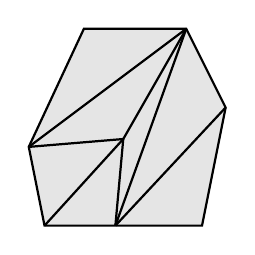
\begin{tikzpicture}
      \coordinate (n1) at (0,0);
      \coordinate (n2) at (2,0);
      \coordinate (n3) at (2.3,1.5);
      \coordinate (n4) at (1.8,2.5);
      \coordinate (n5) at (0.5,2.5);
      \coordinate (n6) at (-0.2,1);
      \coordinate (t0) at (0.9,0);
      \coordinate (t1) at (1,1.1);
      
      \draw[thick,fill=black!10] (n1) -- (n2) -- (n3) -- (n4) -- (n5) -- (n6) -- cycle;
      \draw[thick] (n1) -- (t1);
      \draw[thick] (n6) -- (t1);
      \draw[thick] (n4) -- (t1);
      \draw[thick] (t0) -- (n3);
      \draw[thick] (n4) -- (n6);
      \draw[thick] (t0) -- (t1);
      \draw[thick] (t0) -- (n4);
    \end{tikzpicture} \qquad
    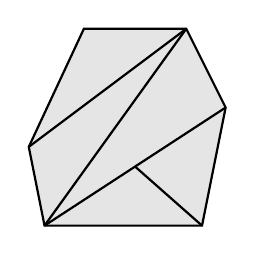
\begin{tikzpicture}
      \coordinate (n1) at (0,0);
      \coordinate (n2) at (2,0);
      \coordinate (n3) at (2.3,1.5);
      \coordinate (n4) at (1.8,2.5);
      \coordinate (n5) at (0.5,2.5);
      \coordinate (n6) at (-0.2,1);
      \coordinate (t0) at (1.15,0.75);
      
      \draw[thick,fill=black!10] (n1) -- (n2) -- (n3) -- (n4) -- (n5) -- (n6) -- cycle;
      \draw[thick] (n1) -- (n3);
      \draw[thick] (n1) -- (n4);
      \draw[thick] (n4) -- (n6);
      \draw[thick] (n2) -- (t0);
    \end{tikzpicture}
  \end{center}
  \caption{The first two pictures show triangulations, while the last picture does not satisfy the second condition of the definition.}
  \label{fig:triangulation-example}
\end{figure}



